\section{Transmission system model}


\begin{frame}{}
    \tableofcontents[currentsection]
\end{frame}



\begin{frame}{Transmission system design}
  Converters are prone to be saturated during short-circuits ($I_{max}$ is reached). 

\begin{table}[!htb]\centering
  \caption{Possible operating states of the converters in grid-following mode.}
  \begin{tabular}{ccc}
    \hline
    \textbf{Converter State} & \textbf{PQ} & \textbf{PV} \\
    \hline
    \hline
    USS & $P$, $Q$ & $P$, $V$ \\
    PSS & $Q$, $I_{max}$ & $V$, $I_{max}$ \\
    FSS & $P=0$, $I_{max}$ & $P=0$, $I_{max}$ \\
    DIS & $P=0$, $Q=0$ & $P=0$, $Q=0$ \\
    \hline
  \end{tabular}
  \label{tab:convs1}
\end{table}

\end{frame}

\subsection{Elements modelling}


\begin{frame}{Elements modelling}
Traditional power flow:
\begin{equation}
  \begin{pmatrix}
    \bm{\Delta f}_P \\
    \bm{\Delta f}_Q \\
  \end{pmatrix} = -
  \begin{pmatrix}
    \frac{d \bm{f}_P}{d \bm{\theta}} & \frac{d \bm{f}_P}{d \bm{\nu}} \\
    \frac{d \bm{f}_Q}{d \bm{\theta}} & \frac{d \bm{f}_Q}{d \bm{\nu}} \\
  \end{pmatrix}
  \begin{pmatrix}
    \bm{\Delta \theta} \\
    \bm{\Delta \nu} \\
  \end{pmatrix}.
  \label{eq:syst2xx}
\end{equation}

Extended Newton-Raphson considering current saturation:
\begin{equation}
  \begin{pmatrix}
    \bm{\Delta f_P} \\
    \bm{\Delta f_Q} \\
    \bm{\Delta f_{I^2}} \\
  \end{pmatrix} = -
  \begin{pmatrix}
    \frac{d \bm{f_P}}{d \bm{\theta}} & \frac{d \bm{f_P}}{d \bm{\nu}} \\
    \frac{d \bm{f_Q}}{d \bm{\theta}} & \frac{d \bm{f_Q}}{d \bm{\nu}} \\
    \frac{d \bm{f_{I^2}}}{d \bm{\theta}} & \frac{d \bm{f_{I^2}}}{d \bm{\nu}} \\
  \end{pmatrix}
  \begin{pmatrix}
    \bm{\Delta \theta} \\
    \bm{\Delta \nu} \\
  \end{pmatrix},
  \label{eq:systfin}
\end{equation}
where the residuals are:
\begin{equation}
  \begin{cases}
    \bm{\Delta f_P} = -\bm{P}_\text{set} + \Re([\bm{V}]\bm{Y}^*\bm{V}^*),\\
    \bm{\Delta f_Q} = -\bm{Q}_\text{set} + \Im([\bm{V}]\bm{Y}^*\bm{V}^*),\\
  \bm{\Delta f}_{I^2} =  \bm{I_c} \bm{I_c}^* = - \bm{I}_{c,max}^2 + (\bm{Y}\bm{V} - [\bm{V}^*]^{-1} \bm{S}^* - \bm{I_l}) \cdot (\bm{Y}\bm{V} - [\bm{V}^*]^{-1} \bm{S}^* - \bm{I}_l)^*.
\end{cases}
\end{equation}
\end{frame}

\begin{frame}{New bus types}
New categories of buses emerge:

\begin{table}[!htb]\centering
  \caption{Traditional types of buses and mapping to new buses depending on the converter state.}
  \begin{tabular}{ccc}
    \hline
    \textbf{Converter State} & \textbf{PQ Control} & \textbf{PV Control} \\
    \hline
    \hline
    USS & PQ & PV \\
    PSS & QI & VI \\
    FSS & PI & PI \\
    DIS & PQ & PQ \\
    \hline
  \end{tabular}
  \label{tab:stat}
\end{table}

\end{frame}



\subsection{Cost modelling}

\begin{frame}{Costs}

\begin{figure}[!htb]\centering
\incfig{texas3}
\caption{Approximate location of the three converters.}
\label{fig:texas}
\end{figure}

\end{frame}


\begin{frame}{Summary}
\begin{table}[!htb]\centering \footnotesize
  \caption{Power flow results for the converters under normal conditions.}
  \begin{tabular}{cccccccc}
    \hline
    \textbf{VSC} & \textbf{State} & $\bm{\nu}$ & $\bm{\theta}$ ($^{\circ}$) & $|\bm{I}|$ & $\bm{P}$ & $\bm{Q}$ & $|\bm{S}|$ \\
    \hline
    \hline
    vsc1 & \cellcolor{gray!40}USS & 1.0073 & -40.7924 & \cellcolor{gray!40}5.8017 & -5.0000 & 3.0260 & 5.8443 \\
    vsc2 & \cellcolor{gray!40}USS & 1.0050 & -63.9565 & \cellcolor{gray!40}1.3882 & -1.0000 & 0.9731 & 1.3953 \\
    vsc3 & \cellcolor{gray!40}USS & 1.0200 & -48.6301 & \cellcolor{gray!40}6.0529 & 6.0000 & 1.4580 & 6.1746 \\
    \hline
  \end{tabular}
  \label{tab:2000_1}
\end{table}

\begin{table}[!htb]\centering \footnotesize
  \caption{Short-circuit results for the converters with $\underline{Z}_f=0.002j$.}
  \begin{tabular}{cccccccc}
    \hline
    \textbf{VSC} & \textbf{State} & $\bm{\nu}$ & $\bm{\theta}$ ($^{\circ}$) & $|\bm{I}|$ & $\bm{P}$ & $\bm{Q}$ & $|\bm{S}|$ \\
    \hline
    \hline
    vsc1 & \cellcolor{gray!40}FSS & 0.0633 & -14.1576 & \cellcolor{gray!40}7.0000 & 0.0000 & 0.4431 & 0.4431 \\
    vsc2 & \cellcolor{gray!40}USS & 0.9997 & -63.3836 & \cellcolor{gray!40}1.3958 & -1.0000 & 0.9732 & 1.3954 \\
    vsc3 & \cellcolor{gray!40}USS & 0.9997 & -46.1701 & \cellcolor{gray!40}6.1764 & 6.0000 & 1.4582 & 6.1746 \\
    \hline
  \end{tabular}
  \label{tab:2000_2}
\end{table}

\begin{table}[!htb]\centering \footnotesize
  \caption{Short-circuit results for the converters with $\underline{Z}_f=0.05j$.}
  \begin{tabular}{cccccccc}
    \hline
    \textbf{VSC} & \textbf{State} & $\bm{\nu}$ & $\bm{\theta}$ ($^{\circ}$) & $|\bm{I}|$ & $\bm{P}$ & $\bm{Q}$ & $|\bm{S}|$ \\
    \hline
    \hline
    vsc1 & \cellcolor{gray!40}PSS & 0.6423 & -34.1962 & \cellcolor{gray!40}7.0000 & -3.1009 & 3.2557 & 4.4962 \\
    vsc2 & \cellcolor{gray!40}USS & 1.0050 & -63.9565 & \cellcolor{gray!40}1.3882 & -1.0000 & 0.9696 & 1.3928 \\
    vsc3 & \cellcolor{gray!40}USS & 1.0200 & -48.6301 & \cellcolor{gray!40}6.0529 & 6.0000 & 1.4453 & 6.1716 \\
    \hline
  \end{tabular}
  \label{tab:2000_3}
\end{table}
\end{frame}

\begin{frame}{Results validation}
 \begin{figure}[!htb]\centering
  \begin{subfigure}{0.45\textwidth}
    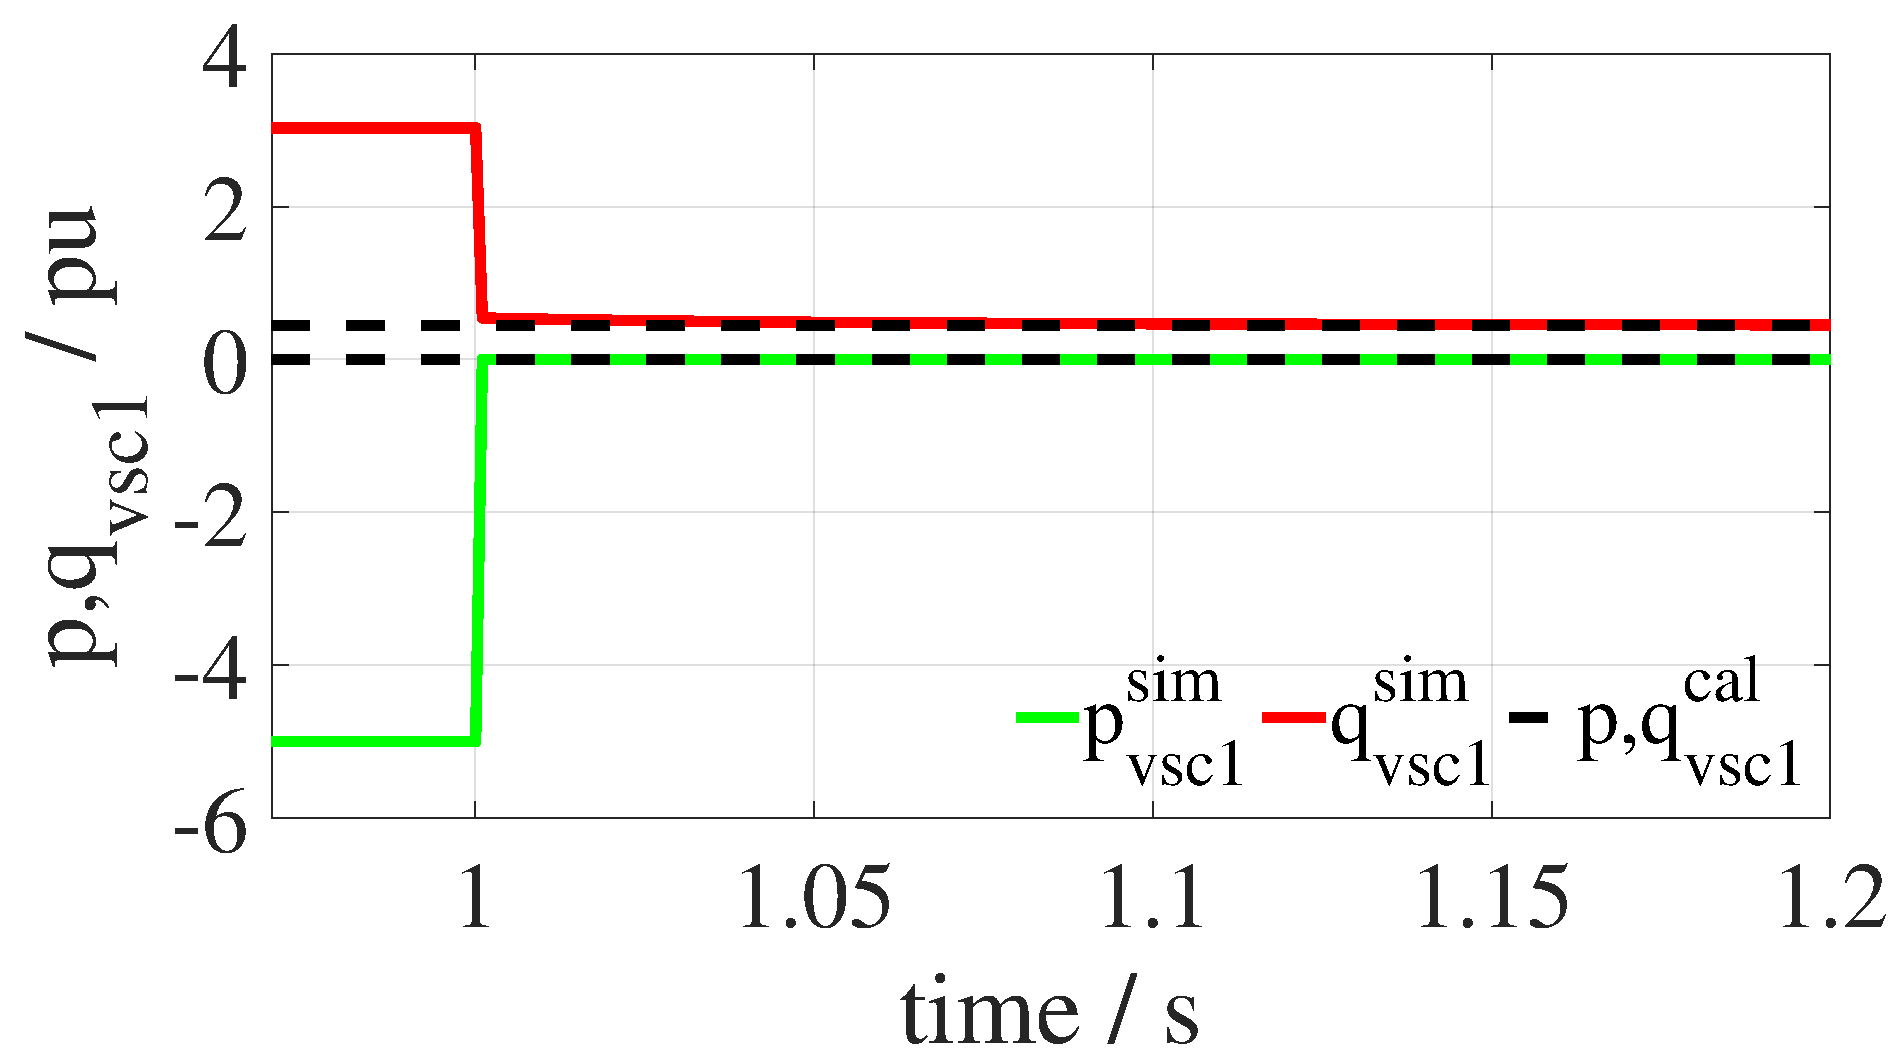
\includegraphics[width=6.0cm]{Data/psim_z0002.pdf}
    \caption{VSC1 power injections.}
  \end{subfigure}
  \begin{subfigure}{0.45\textwidth}
    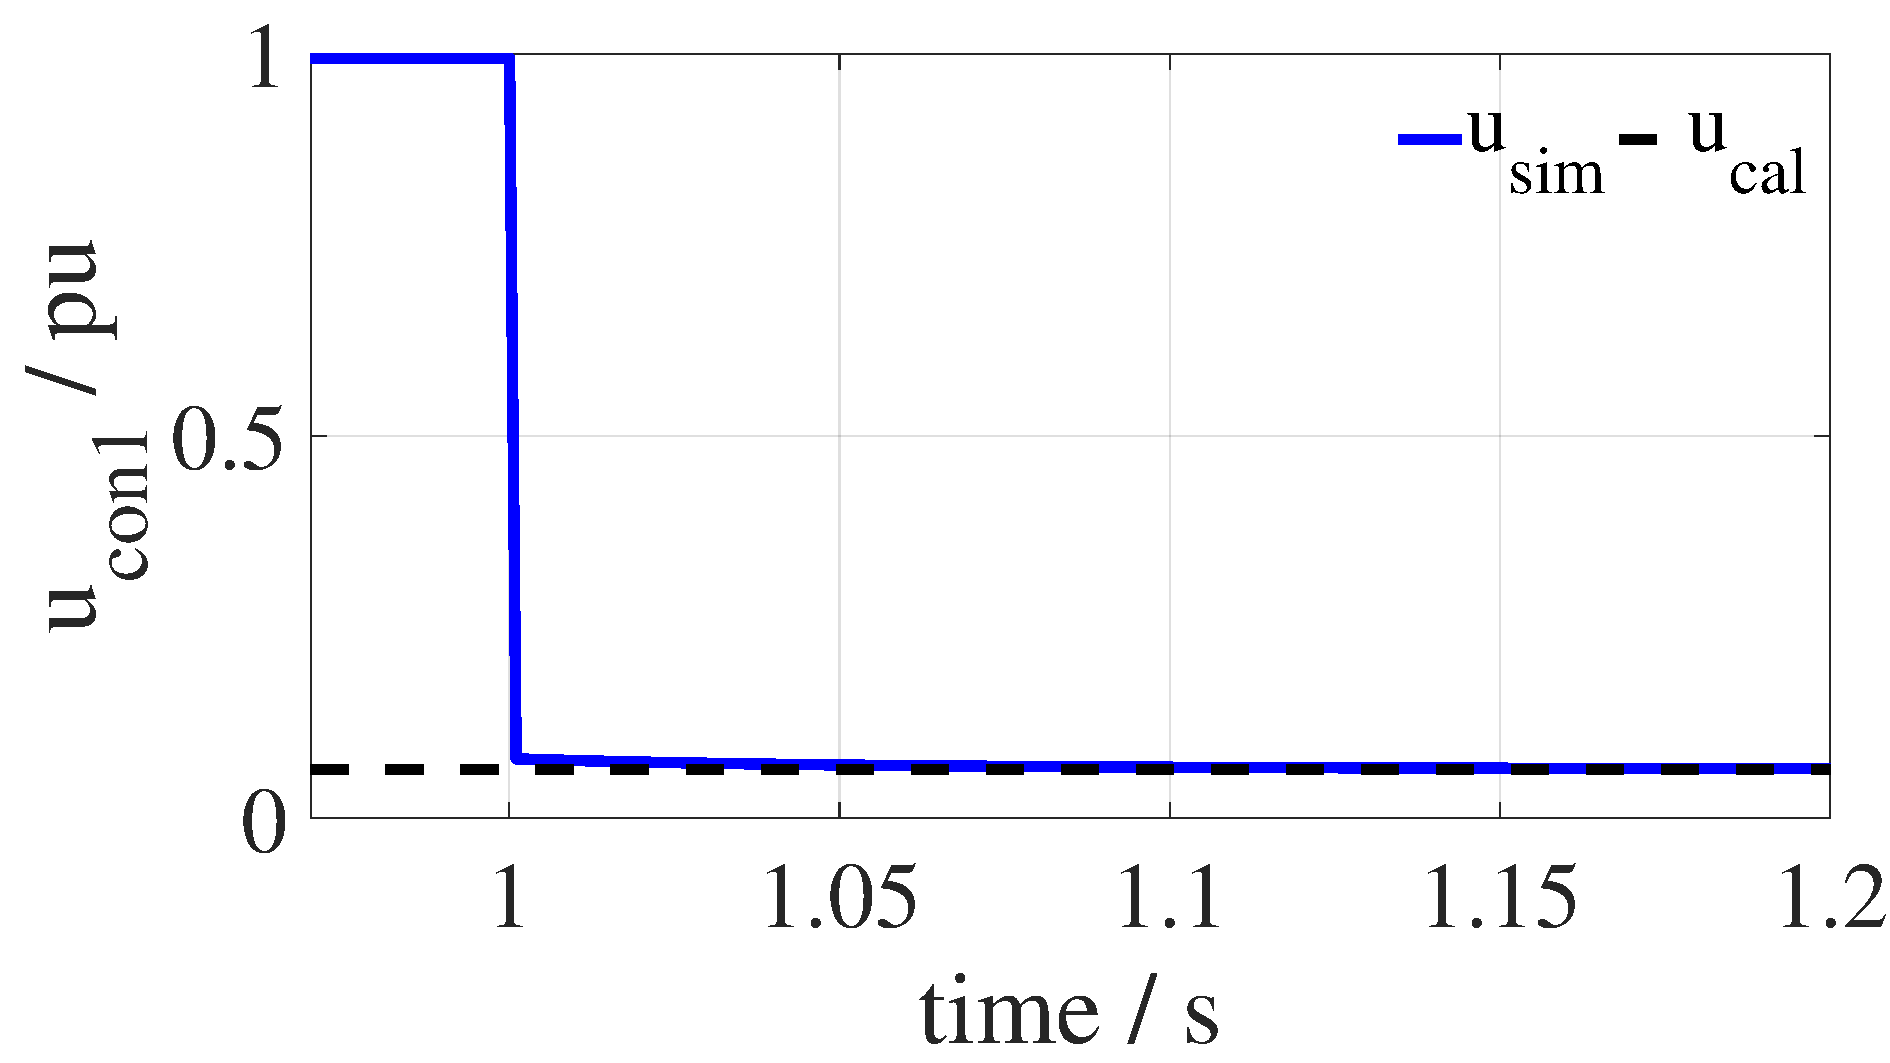
\includegraphics[width=6.0cm]{Data/usim_z0002.pdf}
    \caption{Fault voltage.}
  \end{subfigure}
	\caption{Dynamic simulation with PSS/E for a severe fault with $\underline{Z}_{f}=j0.002$ pu.}
    \label{fig:dyn1}
\end{figure}   
\end{frame}

\begin{frame}{Comparison with PSS/E}
  Steady-state calculations:
\begin{table}[!htb]\centering\footnotesize
	\caption{Steady-state short-circuit results with the proposed method and PSS/E.}
	\begin{tabular}{cccc}
        \hline
        \backslashbox{$\bm{\underline{Z}_{f}}$}{$\bm{I_{sc}}$} & \textbf{Proposed method} & \textbf{PSS/E VSCs as generators} & \textbf{PSS/E VSCs as FACTS} \\
        \hline
        \hline
        $j0.05$ & \cellcolor{green!30}12.75 & \cellcolor{red!30}13.40 & \cellcolor{red!30}12.17 \\
		$j0.002$ & \cellcolor{green!30}31.40 & \cellcolor{red!30}32.57 & \cellcolor{red!30}25.91 \\
        \hline
	\end{tabular}
	\label{tab:valid}
\end{table}
PSS/E dynamic simulation:
	\begin{table}[!htb]\centering\footnotesize
			\caption{Comparison of efficiency with PSS/E dynamic simulation.}
			% \begin{tabular}{m{3cm}<{\centering}|m{2.5cm}<{\centering}m{4cm}<{\centering}}
              \begin{tabular}{crr}
              \hline
              $\bm{t_{sim}}$ \textbf{after fault (s)}& \textbf{Calculation time (s)}& \textbf{Error} $|\bm{u_{sample}-u_{cal}}|$ \textbf{(pu)} \\
                \hline
                \hline
				0.3 & 1.43 & $42 \times 10^{-3}$ \\
				1 & 3.52 & $19.8 \times 10^{-3}$ \\
				2 & 6.81 & $6.5 \times 10^{-3}$ \\
				3 & 10.07 & $1.6 \times 10^{-3}$ \\
				4 & 13.14 & $<0.1 \times 10^{-3}$ \\
				\hline
                \rowcolor[gray]{0.8} Proposed method & 0.085 & $6.17 \times 10^{-11}$ \\
                \hline
			\end{tabular}
            \label{tab:comparex}
	\end{table}	

\end{frame}

% \subsection{Algebraic limits}
% \begin{frame}{Algebraic limits}
% \begin{itemize}
%     \item Up to this point, the states of converters are predetermined. 
%     \item Converters are initially assumed to be unsaturated. If no solution is obtained, they are saturated following some heuristics.
%     \item Finding a solution is not guaranteed, and multiple solutions can coexist.
%     \item Since each of the $n$ converters can operate in 4 different states (USS, PSS, FSS and DIS), there are $4^n$ possible combinations. Solving systems with many converters is a computational challenge.
% \end{itemize}
% For all these reasons, it may be a good idea to include the current limits of the converters in an algebraic manner. The system of equations could be solved at one go. 
% \end{frame}

% \begin{frame}{Formulation of the Lagrangian}
% \begin{figure}[!htb]\centering\footnotesize
%   \begin{circuitikz}[european]
%     \draw[line width=0.1cm] (0,0) to [short] (0,-0.8);
%     \draw (0,-0.4) to [/tikz/circuitikz/bipoles/length=25pt, R] (2,-0.4);
%     \draw (0,-0.2) to [/tikz/circuitikz/bipoles/length=25pt, R, l=${g}_{ij}$] (2,0.6);
%     \draw (0,-0.6) to [/tikz/circuitikz/bipoles/length=25pt, R] (2,-1.4);
%     \draw (-0.5,-0.6) to [short] (-0.0,-0.6);
%     % \draw (-0.2,-0.6) to [/tikz/circuitikz/bipoles/length=25pt, R, l_=$\underline{Y}_{sh,i}$] (-0.2,-2.5);
%   \draw (-0.5,-1) to [short, i=${I}_i$] (-0.5,-0.6);
%     \draw (-0.5,-2.5) to [american current source] (-0.5,-1.0);
%     \draw (-0.7,-2.5) to [short] (-0.3,-2.5);
%     % \draw (-2.2,-0.4) to [sdcac] (-1.2,-0.4);
%     % \draw (0,0) to [twoportsplit, t1={$=$}, t2={$=$}] ++(3,0);

%     \draw (0.4,-1) to [/tikz/circuitikz/bipoles/length=25pt, R, l=$g_{sh,i}$] (0.4,-2.4);
%     \draw (0.4, -2.4) to [short] (0.4,-2.5);
%     \draw (0.2,-2.5) to [short] (0.6,-2.5);
%     \draw (0.4,-1) to [short] (0,-0.6);

%     \draw (-2.2,-0.9) to [short] (-1.2,-0.9);
%     \draw (-1.2,0.1) to [short] (-2.2,0.1);
%     \draw (-2.2,-0.9) to [short] (-2.2,0.1);
%     \draw (-1.2,-0.9) to [short] (-1.2,0.1);
%     \draw (-2.2,0.1) to [short] (-1.2,-0.9);

%     \draw (-1.5, -0.1) to [short] (-1.3, -0.1);
%     \draw (-1.5, 0.0) to [short] (-1.3, 0.0);

%     \draw (-2.1, -0.8) to [short] (-1.9, -0.8);
%     \draw (-2.1, -0.7) to [short] (-1.9, -0.7);

%     \draw (-1.2,-0.4) to [short, i=${P}_{i}$] (-0.0, -0.4);
%     \node[] at (0,0.2) {${V}_i$};

%     \draw[line width=0.1cm] (2,0.6) to [short] (2.1,0.37);
%     \draw[line width=0.1cm] (2,0.6) to [short] (1.9,0.83);

%     \draw[line width=0.1cm] (2,-1.4) to [short] (2.1,-1.17);
%     \draw[line width=0.1cm] (2,-1.4) to [short] (1.9,-1.63);

%     \draw[line width=0.1cm] (2,-0.4) to [short] (2,-0.65);
%     \draw[line width=0.1cm] (2,-0.4) to [short] (2,-0.15);

%     \node[] at (2,1.0) {$j$};
%     \node[] at (2,0.0) {$j+1$};
%     \node[] at (2,-1) {$j+2$};

%   \end{circuitikz}
%   \caption{Scheme of a DC bus with a converter.}
%   \label{fig:rep1}
% \end{figure}

% The current balance and the associated Lagrangian are:
% \begin{equation}
%   \mathcal{F} = \sum_j g_{ij}(V_i - V_j) + V_i g_{sh,i} - \frac{P_i}{V_i} - I_i = 0,
% \end{equation}
% \begin{equation}
%   \mathcal{L} = \int \mathcal{F} d\{V_i\} = \frac{1}{2}\sum_i \sum_{j<i} g_{ij}(V_i - V_j)^2 + \frac{1}{2}\sum_i V_i^2 g_{sh,i} - \sum_i P_i \ln V_i - \sum_i I_iV_i.
% \end{equation}
% \end{frame}

% \begin{frame}{Formulation of the Lagrangian}
% The minimization problem is:
% \begin{equation}
% \begin{aligned}
%   \min_{\{V_i\}} \quad & \frac{1}{2}\sum_i \sum_{j<i} g_{ij}(V_i - V_j)^2 + \frac{1}{2}\sum_i V_i^2 g_{sh,i} - \sum_i P_i \ln V_i - \sum_i I_iV_i, \\
%   \textrm{s.t.} \quad & V_i^{sp} - V_i = 0, \\
%                       & I_i^\text{min} \leq I_i \leq I_i^\text{max}. \\
% \end{aligned}
% \end{equation}

% The dual problem with barrier functions becomes:
% \begin{equation}
% \begin{aligned}
%   \begin{split}
%     \max_{\{I_i\}} \quad & \frac{1}{2}\sum_i \sum_{j<i} g_{ij}(V_i - V_j)^2 + \frac{1}{2}\sum_i V_i^2 g_{sh,i} - \sum_i P_i \ln V_k - \sum_i I_i(V_i - V_i^{sp}) \\
%                        &+ \mu_1 \ln{(I_i^\text{max} - I_i)} + \mu_2 \ln{(I_i - I_i^\text{min})}.
%   \end{split}
% \end{aligned}
% \label{eq:iffinal}
% \end{equation}
% Deriving it with respect to $I_i$ yields the equation of interest:
% \begin{equation}
%   -(V_i - V_i^{sp})(I_i^\text{max} - I_i)(I_i - I_i^\text{min}) - \mu(I_i - I_i^\text{min}) + \mu(I_i^\text{max} - I_i) = 0.
%   \label{eq:iok}
% \end{equation}

% \end{frame}


% \begin{frame}{Results for a simple DC system}
% The initial results are:
% \begin{table}[!htb]\centering\footnotesize
%   \caption{Results for the DC power flow base case.}
%   \begin{tabular}{cc}
%     \hline
%     \textbf{Magnitude} & \textbf{Value}\\
%     \hline
%     \hline
%     $V_1$ & 1.0100 \\
%     $P_1$ & 0.4703 \\
%     $V_2$ & 0.9867 \\
%     $P_3$ & 0.0406 \\
%     \hline
%   \end{tabular}
%   \label{tab:r1}
% \end{table}
% And the results obtained by thightening the current limits turn out to be:
% \begin{table}[!htb]\centering\footnotesize
%   \caption{DC power flow results considering current limits of $\pm 0.4$.}
%   \begin{tabular}{cc}
%     \hline
%     \textbf{Magnitude} & \textbf{Value}\\
%     \hline
%     \hline
%     $V_1$ & 1.0012 \\
%     $I_1$ & 0.4000 \\
%     $V_2$ & 0.9812 \\
%     $P_3$ & 0.1084 \\
%     \hline
%   \end{tabular}
%   \label{tab:r3}
% \end{table}
% \end{frame}
